\section{方法B\label{方法B}}

\begin{figure}[htb]
    \centering
    \subfloat{
        \includegraphics[width=0.45\linewidth]{P1.jpg}
    }%\hfill
    \subfloat{
        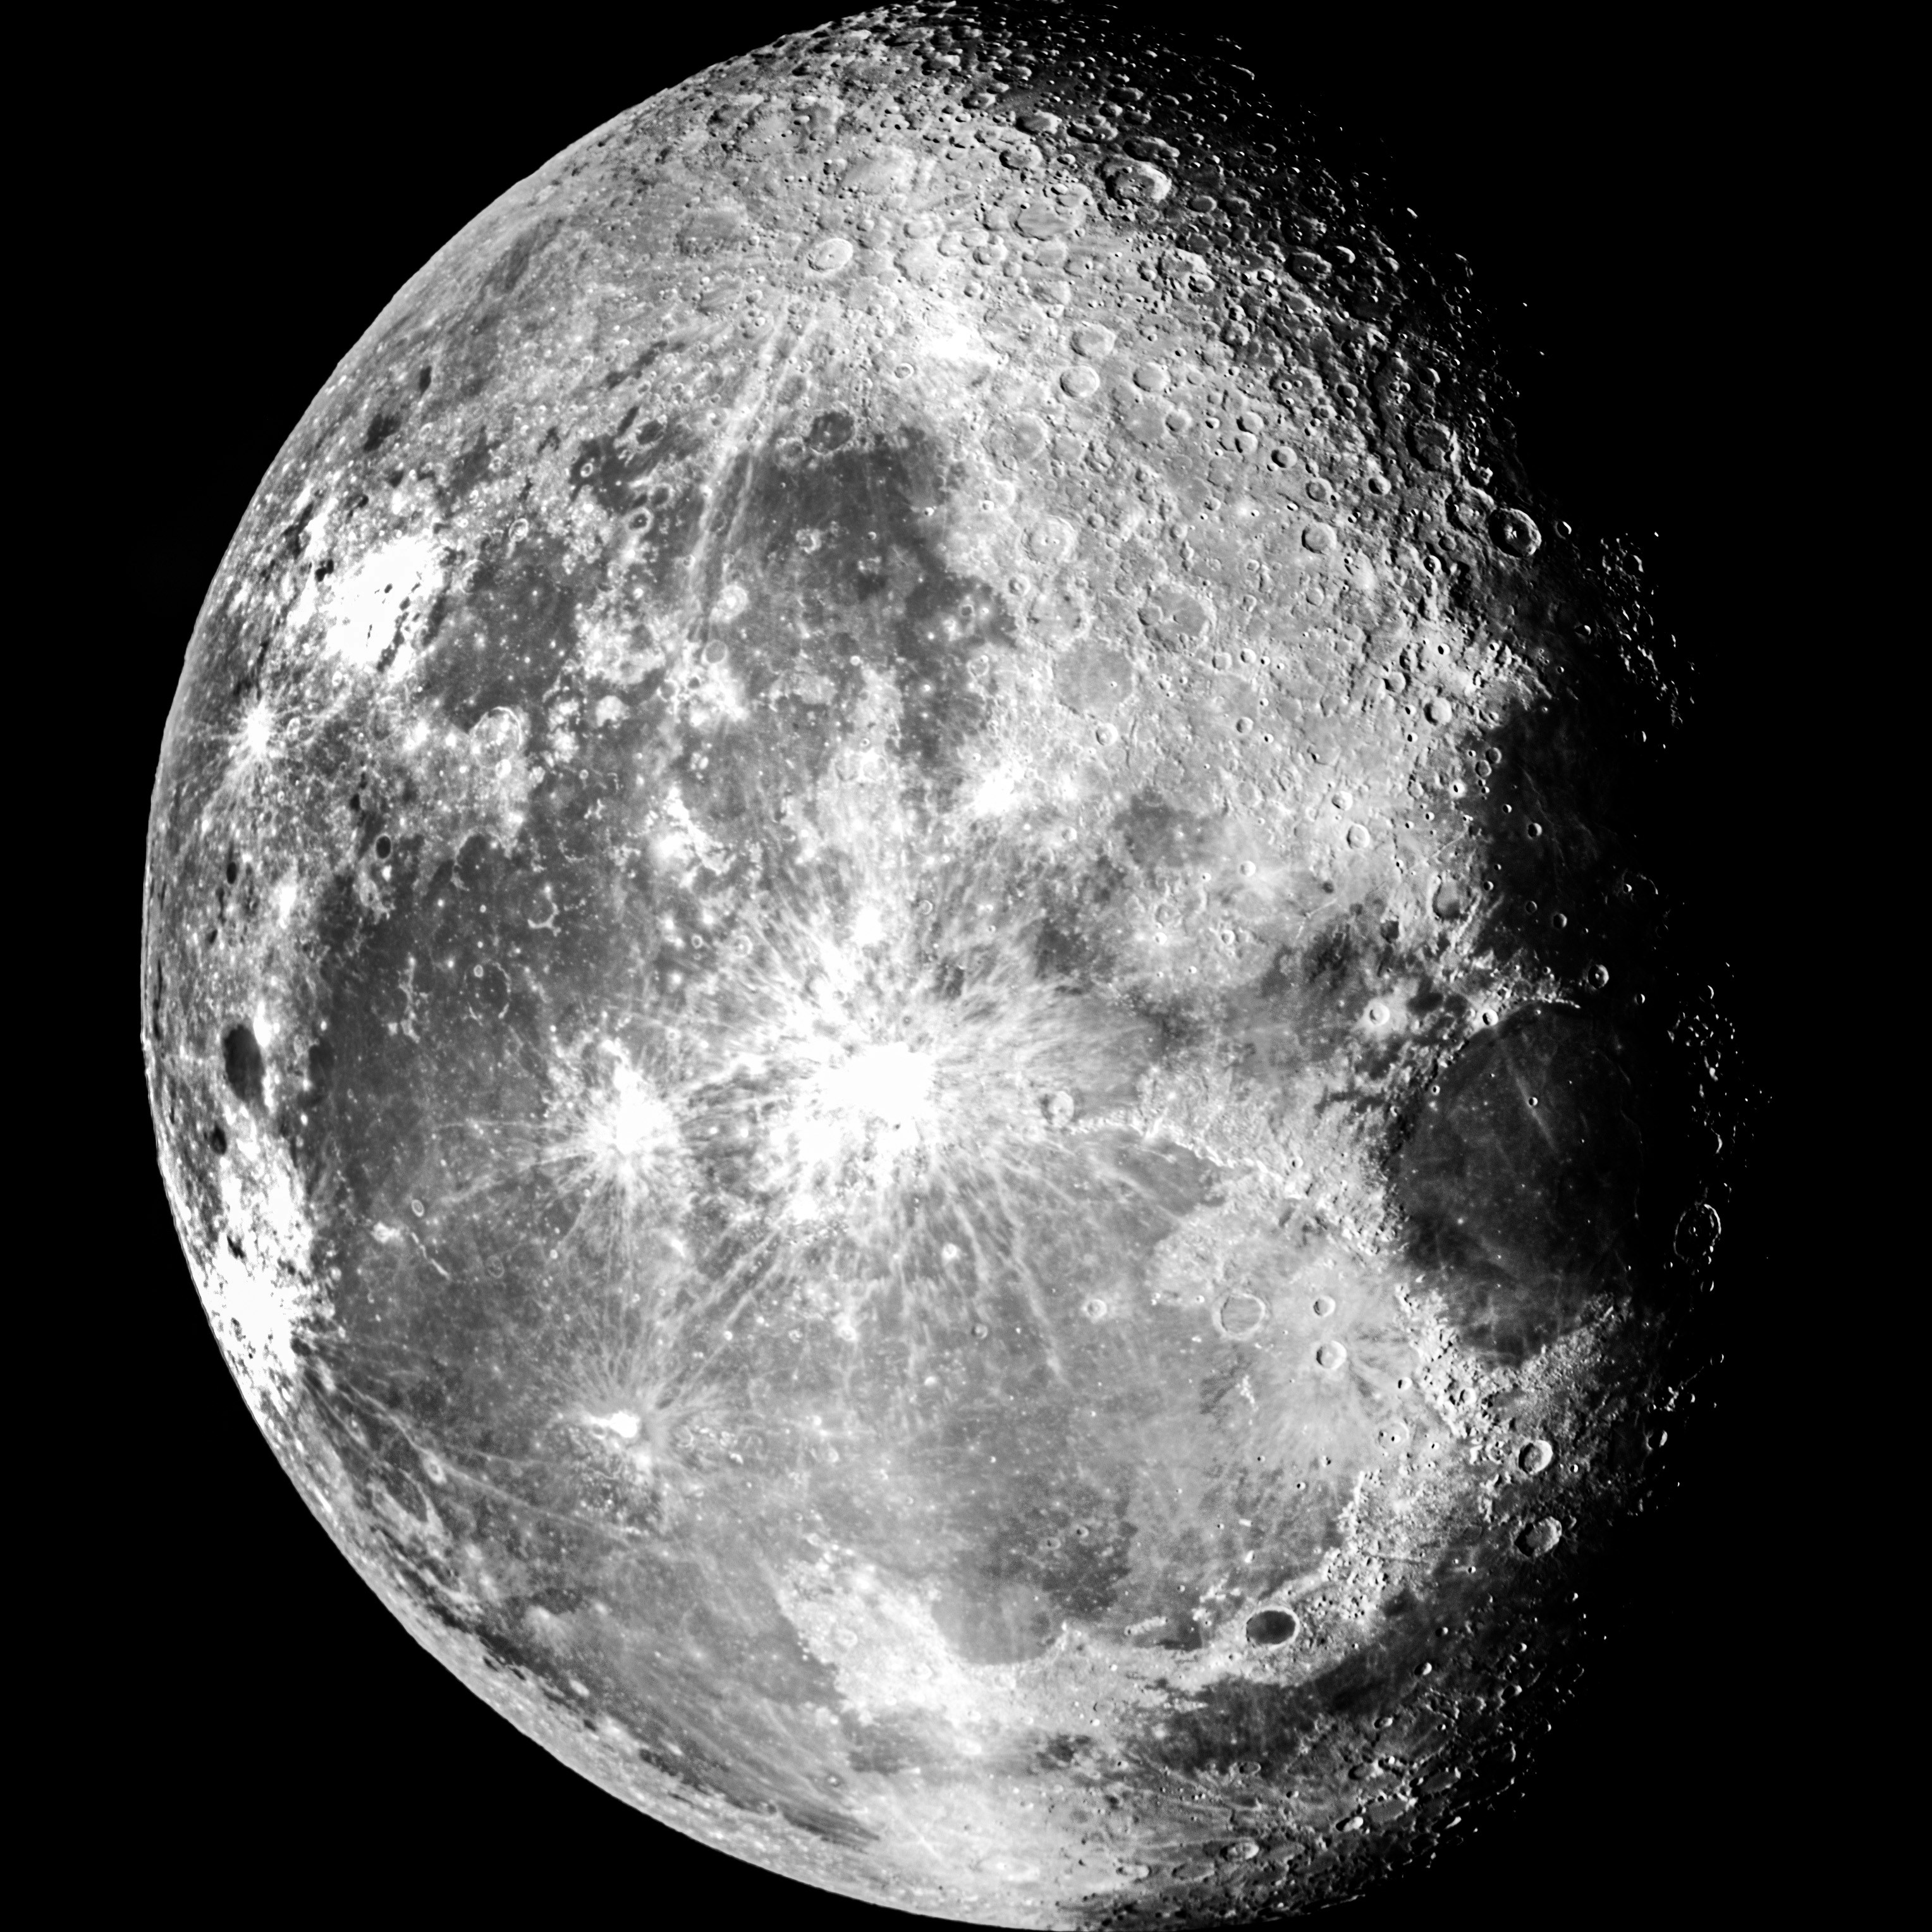
\includegraphics[width=0.45\linewidth]{P2.jpg}
    }\\
    \captionsetup{font=footnotesize}
    \bicaption{一些有关图片的描述。}{Some descriptions of the pictures in question.}
    \label{fig:幂律参数空间B}
\end{figure}

\subsection{方法B的二级标题}

方法B二级标题的正文,方法B二级标题的正文,方法B二级标题的正文,方法B二级标题的正文,方法B二级标题的正文。

\subsubsection{方法B的三级标题}

方法B三级标题的正文,方法B三级标题的正文,方法B三级标题的正文,方法B三级标题的正文,方法B三级标题的正文。


% Please add the following required packages to your document preamble:
% \usepackage{booktabs}
\begin{table}[htb]
    \centering
    \captionsetup{font=footnotesize}
    \bicaption{符号对照表}{Symbol cross-reference table}
    \label{tab:符号对照表B}
    \begin{tabular}{@{}cc@{}}
        \toprule
        符号     & 含义       \\ 
        \midrule
        $a$     & 尺度因子    \\
        $k$     & 波尔兹曼常数 \\
        $T_c$   & 一些描述    \\
        $\beta$ & 一些描述    \\
        $t_b$   & 一些描述    \\
        \bottomrule
    \end{tabular}
\end{table}

\subsection{方法B的二级标题}

方法B二级标题的正文,方法B二级标题的正文,方法B二级标题的正文,方法B二级标题的正文,方法B二级标题的正文。

\subsubsection{方法B的三级标题}

方法B三级标题的正文,方法B三级标题的正文,方法B三级标题的正文,方法B三级标题的正文,方法B三级标题的正文。